\documentclass{article}
\usepackage[italian]{babel}
\usepackage[utf8]{inputenc}
\usepackage{listingsutf8}
\usepackage[margin=75pt]{geometry}
\usepackage{amsmath}
\usepackage{graphicx}
\usepackage{spverbatim}
%\usepackage{verbatim}
%\usepackage{fancyvrb}
\usepackage{hyperref}

%IMPORT CODE
%\usepackage{minted}
\usepackage{listings}
\usepackage{color}

\definecolor{dkgreen}{rgb}{0,0.6,0}
\definecolor{gray}{rgb}{0.5,0.5,0.5}
\definecolor{mauve}{rgb}{0.58,0,0.82}

\lstset{frame=tb,
	language=Haskell,
	aboveskip=3mm,
	belowskip=3mm,
	showstringspaces=false,
	columns=flexible,
	basicstyle={\small\ttfamily},
	numbers=none,
	numberstyle=\tiny\color{gray},
	keywordstyle=\color{blue},
	commentstyle=\color{dkgreen},
	stringstyle=\color{mauve},
	breaklines=true,
	breakatwhitespace=true,
	tabsize=3
}

% in way to comment a block
\long\def\/*#1*/{}

\title{\textbf{Relazione sul Progetto d'Esame}}
\author{Francesco Rombaldoni}
\date{\small Università degli Studi di Urbino Carlo Bo\\
	Insegnamento di Programmazione Logica e Funzionale}

\begin{document}
	\maketitle
	
%	Prepared for a formal document
%	\newpage
	
	%\tableofcontents
	%\newpage
\newpage

\section{Specifica del Problema}
Scrivere un programma Haskell e un programma Prolog che, dato l'inserimento di due rilevamenti satellitari in formato di coordinata unica nella quale la latitudine e la longitudine sono rappresentate in formato D.M.G internazionale, effettuano le seguenti operazioni: controllare la validità dei rilevamenti inseriti dall'utente, calcolare e riportare (sempre in formato di coordinata unica) per ogni rilevamento la corrispettiva latitudine e longitudine in formato decimale, calcolare e riportare la distanza in chilometri compresa tra i due rilevamenti satellitari, calcolare e riportare l'angolo di rotta espresso in gradi (sia diretto che inverso) che unisce i due rilevamenti inseriti.
\newline
\newline
%\emph{[Confrontare lo svolgimento delle fasi successive con quanto riportato nelle prossime pagine.]}\\
\newpage
			
\section{Analisi del Problema}
\subsection{Dati di Ingresso del Problema}
Per ciascuna delle quattro operazioni, i dati d'ingresso del problema sono rappresentati da due diversi rilevamenti satellitari in formato di coordinata unica nella quale la latitudine e la longitudine sono rappresentate in formato D.M.G internazionale. \\
Esempio di rilevamento accettato: N 40 45 36.000 - E 073 59 02.400

\subsection{Dati di Uscita del Problema}
Per ogni inserimento di una coppia di rilevamenti nel formato prima specificato i dati d'uscita del problema, rispettivamente alle ultime tre operazioni descritte all'interno della sezione di specifica del problema, sono: il risultato della conversione delle coordinate del primo rilevamento inserito dal formato D.M.G internazionale a quello decimale, il risultato della conversione delle coordinate del secondo rilevamento inserito dal formato D.M.G internazionale a quello decimale, il risultato del calcolo della distanza compresa tra i due rilevamenti inseriti, il risultato del calcolo dell'angolo di rotta diretto che unisce i due rilevamenti, il risultato del calcolo dell'angolo di rotta inverso che unisce i due rilevamenti.\\ 
L'operazione di controllo della validità dei rilevamenti immessi restituisce un messaggio d'errore nel caso in cui i rilevamenti inseriti non risultino validi. Il messaggio d'errore è composto da due parti, dove nella prima parte viene descritto il tipo d'errore commesso, nella seconda viene riportata la porzione di coordinata nella quale è stato rilevato l'errore. 

\subsection{Relazioni Intercorrenti tra i Dati del Problema}
Dato l'inserimento di due rilevamenti nel formato prima specificato, le operazioni in questione sono definite come segue:
\begin{itemize}
	\item Controllo della validità dei rilevamenti; per ogni rilevamento inserito, si verifica che la sua lunghezza sia quella di un rilevamento standard in formato D.M.G internazionale non abbreviato (ovvero un rilevamento nel quale il numero di cifre che compone un valore rimane costante), si verifica che il suo formato sia corretto (controllando se la posizione degli spazi all'interno della "stringa" rappresentante il rilevamento sia corretta) ed infine si verifica che le coordinate inserite siano reali. 
	
	\item Conversione delle coordinate dalla forma D.M.G internazionale alla forma decimale; data una qualsiasi coordinata il passaggio dalla forma D.M.G internazionale alla forma decimale è definito come segue: \\
	Decimale = (Gradi + (((Secondi / 60) + Primi) / 60) * (-1) se il Segno è  S o W).
	
	\item Calcolo della distanza compresa tra due rilevamenti;  data una coppia di rilevamenti convertiti in formato decimale rispettivamente denominati "A" e "B" la loro distanza compresa è definita come: \\
	$Distanza(A, B) = R * \arccos(\sin(latA * \pi / 180) * \sin(latB * \pi / 180) + \cos(latA * \pi / 180) * \cos(latB * \pi / 180) * \cos((lonA - lonB) * \pi / 180)). $\\
	Dove R rappresenta il raggio della Terra.
	
	\item Calcolo dell'angolo di rotta diretto e inverso tra due rilevamenti; data una coppia di rilevamenti convertiti in formato decimale rispettivamente denominati "A" e "B" e data la condizione che la latitudine e la longitudine siano diverse, l'angolo di rotta diretto e inverso compresa tra i rilevamenti è definita come: \\
	$\Delta\Phi = \ln( \tan(latB * \pi / 360 + \pi / 4 ) / \tan(latA * \pi / 360 + \pi / 4 )). $\\
	$ \Delta Lon = abs(lonA - lonB). $ \\
	$ Angolo Diretto = atan2((\Delta Lon * \pi / 180), (abs(\Delta\Phi))) / \pi * 180. $\\
	$ Angolo Inverso = Angolo Diretto + 180.$\\
	Nel caso in cui le latitudini dei due rilevamenti siano identiche:\\
	$\Delta\Phi = \pi / 180 * 0.000000001.$\\
	Nel caso in cui le longitudini dei due rilevamenti siano identiche:\\
	$\Delta Lon = \pi / 180 * 0.000000001.$\\
\end{itemize}
\newpage

\section{Progettazione dell'Algoritmo}
\subsection{Scelte di Progetto}
Il rilevamento immesso dall'utente è rappresentato sotto forma di "stringa", pertanto il rilevamento è gestibile come una lista di caratteri di tipo "char". Le varie parti d'interesse sulla lista, vengono estratte a delle posizioni precise (per esempio si suppone che il segno della prima coordinata si trovi nella posizione uno della lista).  Siccome le informazioni vengono estratte dalla lista a delle posizioni precedentemente stabilite (quindi senza controllare la presenza di simboli per la ricerca delle parti d'interesse sulla lista), si controlla che quest'ultima sia precisamente di trentadue caratteri (considerando anche gli spazi) e nel formato corretto.\\
Un'ulteriore decisione architetturale è stata presa nella gestione delle singole coordinate, infatti la latitudine e la longitudine individuate all'interno della lista di caratteri "char" vengono convertite rispettivamente in due "tuple" definite come segue: (Char, Integer, Integer, Float) ovvero (Segno, Gradi, Primi, Secondi), in modo da poter semplificare l'implementazione delle funzioni/predicati atti alla conversione delle coordinate dal formato D.M.G internazionale al formato decimale. Nel caso specifico del programma Prolog al posto delle "tuple" vengono utilizzate delle liste formate da elementi "atomici" definite come segue:  [Segno, Gradi, Primi, Secondi].
 
\subsection{Passi dell'Algoritmo}
%I passi dell'algoritmo sono diversi a seconda del tipo d'operazione:
\begin{enumerate}
	\item Acquisizione del primo rilevamento.
	\item Acquisizione del secondo rilevamento.
	\item Verifica se i due rilevamenti acquisiti siano differenti.
	
	\item Controllo della validità dei rilevamenti:
	\begin{enumerate}
		\item La "stringa" contenente il rilevamento inserito dall'utente viene convertita in una lista di caratteri "char".
		\item Viene valutato se la lista così ottenuta sia composta da trentadue elementi e nel formato corretto verificando che gli spazi siano posizionati nelle  seguenti posizioni della lista: 2, 5, 8, 15, 17, 19, 23, 25. Nel caso in cui la lista non possieda trentadue elementi oppure i caratteri di spazio non siano posizionati correttamente viene restituito un messaggio d'errore.
		\item La lista viene manipolata per estrarre le informazioni relative alla latitudine da inserire nella "tupla"/lista che rappresenta la latitudine in formato D.M.G internazionale.
		\item La lista viene nuovamente manipolata per estrarre le informazioni relative alla longitudine da inserire nella "tupla"/lista che rappresenta la longitudine in formato D.M.G internazionale.
		\item Si esegue la verifica delle informazioni contenute all'interno della "tupla"/lista rappresentante la latitudine in formato D.M.G internazionale, verificando nel seguente ordine:  la correttezza del "segno" controllando che sia "N" oppure "S", i "gradi" controllando che siano compresi tra il valore zero ed il valore ottantanove (estremi compresi), i "primi" ed i "secondi" controllando che entrambi i valori siano compresi tra il valore zero ed il valore cinquantanove (estremi compresi). Nel caso in cui uno dei quattro controlli dovesse rilevare un errore, viene restituito un messaggio nel quale si descrive il tipo d'errore riscontrato.
		\item Si esegue la verifica delle informazioni contenute all'interno della "tupla"/lista rappresentante la longitudine in formato D.M.G internazionale, verificando nel seguente ordine:  la correttezza del "segno" controllando che sia "E" oppure "W", i "gradi" controllando che siano compresi tra il valore zero ed il valore centosettantanove (estremi compresi), i "primi" ed i "secondi" controllando che entrambi i valori siano compresi tra il valore zero ed il valore cinquantanove (estremi compresi). Nel caso in cui uno dei quattro controlli dovesse rilevare un errore, viene restituito un messaggio nel quale si descrive il tipo d'errore riscontrato.
	\end{enumerate}

	\item Conversione delle coordinate dalla forma D.M.G internazionale alla forma decimale:
	\begin{enumerate}
		\item La "tupla"/lista contenente la latitudine in formato D.M.G internazionale viene convertita in formato decimale applicando la seguente formula: \\Decimale = (Gradi + (((Secondi / 60) + Primi) / 60) * (-1) se il Segno è  S). 
		\item La "tupla"/lista contenente la longitudine in formato D.M.G internazionale viene convertita in formato decimale applicando la seguente formula: \\Decimale = (Gradi + (((Secondi / 60) + Primi) / 60) * (-1) se il Segno è  W).
		\item Le coordinate così ottenute vengono riunite all'interno di una "tupla"/lista così definita: (latitudine decimale, longitudine decimale)/[latitudine decimale, longitudine decimale].
		\item Stampa a video della latitudine in formato decimale e della longitudine in formato decimale.
	\end{enumerate}

	\item Calcolo della distanza compresa tra i due rilevamenti inseriti: 
	\begin{enumerate}
		\item Data una coppia di rilevamenti in formato decimale rispettivamente denominati "A" e "B", la distanza compresa tra i due rilevamenti viene calcolata applicando la seguente formula: \\$Distanza(A, B) = R * \arccos(\sin(latA * \pi / 180) * \sin(latB * \pi / 180) + \cos(latA * \pi / 180) * \cos(latB * \pi / 180) * \cos((lonA - lonB) * \pi / 180)). $
		\item Stampa a video della distanza compresa tra la coppia di rilevamenti dati.
	\end{enumerate}

	\item  Calcolo dell'angolo di rotta diretto e inverso tra i due rilevamenti inseriti:
	\begin{enumerate}
		\item  Si considera una coppia di rilevamenti in formato decimale rispettivamente denominati "A" e "B".
		\item Si calcola il $\Delta\Phi$ dei rilevamenti nel caso in cui le latitudini dei suddetti siano diverse applicando la seguente formula:\\ $\Delta\Phi = \ln( \tan(latB * \pi / 360 + \pi / 4 ) / \tan(latA * \pi / 360 + \pi / 4 )). $\\
		Nel caso in cui le latitudini dei due rilevamenti siano identiche, il $\Delta\Phi$ viene calcolato in questo modo:\\ $\Delta\Phi = \pi / 180 * 0.000000001.$
		\item Si calcola il $\Delta Lon$ dei rilevamenti nel caso in cui le longitudini dei suddetti siano diverse applicando la seguente formula:\\ $ \Delta Lon = abs(lonA - lonB). $\\
		Nel caso in cui le longitudini dei due rilevamenti siano identiche, il $\Delta Lon$ viene calcolato in questo modo:\\ $\Delta Lon = \pi / 180 * 0.000000001.$
		\item Si calcola quindi l'angolo di rotta diretto tra i due rilevamenti applicando la seguente formula:\\ $ Angolo Diretto = atan2((\Delta Lon * \pi / 180), (abs(\Delta\Phi))) / \pi * 180.$\\
		\item L'angolo di rotta inverso tra i due rilevamenti è calcolato applicando la seguente formula: \\ $ Angolo Inverso = Angolo Diretto + 180.$\\
		\item Stampa a video dell'angolo di rotta diretto tra i due rilevamenti considerati.
		\item Stampa a video dell'angolo di rotta inverso tra i due rilevamenti considerati.
	\end{enumerate}

\end{enumerate}
\newpage

\section{Implementazione dell'Algoritmo}
\raggedright
\underline{File sorgente \textbf{Detection.hs:}}
\lstinputlisting[language=Haskell]{../Haskell/Detection.hs}

\underline{File sorgente \textbf{Properties.hs:}}
\lstinputlisting[language=Haskell]{../Haskell/Properties.hs}

\underline{File sorgente \textbf{Tools.hs:}}
\lstinputlisting[language=Haskell]{../Haskell/Tools.hs}

\lstset{inputencoding=utf8/latin1}
\underline{File sorgente \textbf{Main.hs:}}
\lstinputlisting[language=Haskell]{../Haskell/Main.hs}

\newpage
\raggedright
\underline{File sorgente \textbf{Detection.pl:}}
\lstinputlisting[language=Prolog]{../Prolog/Detection.pl}

\underline{File sorgente \textbf{Properties.pl:}}
\lstinputlisting[language=Prolog]{../Prolog/Properties.pl}

\underline{File sorgente \textbf{ListTools.pl:}}
\lstinputlisting[language=Prolog]{../Prolog/ListTools.pl}

\lstset{inputencoding=utf8/latin1}
\underline{File sorgente \textbf{Main.pl:}}
\lstinputlisting[language=Prolog]{../Prolog/Main.pl}
\newpage

\section{Testing del Programma}
\subsection*{Test Haskell 1}

\lstset{inputencoding=utf8/latin1}
\lstinputlisting[language=]{Haskell_Tests/1-Duplicate_Detections.sh}

\subsection*{Test Haskell 2}

\lstset{inputencoding=utf8/latin1}
\lstinputlisting[language=]{Haskell_Tests/2-String_Formatting.sh}

\subsection*{Test Haskell 3}

\lstset{inputencoding=utf8/latin1}
\lstinputlisting[language=]{Haskell_Tests/3-Check_Sign.sh}

\subsection*{Test Haskell 4}

\lstset{inputencoding=utf8/latin1}
\lstinputlisting[language=]{Haskell_Tests/4-Check_Sign.sh}

\subsection*{Test Haskell 5}

\lstset{inputencoding=utf8/latin1}
\lstinputlisting[language=]{Haskell_Tests/5-Check_Sign.sh}

\subsection*{Test Haskell 6}

\lstset{inputencoding=utf8/latin1}
\lstinputlisting[language=]{Haskell_Tests/6-Check_Degrees.sh}

\subsection*{Test Haskell 7}

\lstset{inputencoding=utf8/latin1}
\lstinputlisting[language=]{Haskell_Tests/7-Check_Primes.sh}

\subsection*{Test Haskell 8}

\lstset{inputencoding=utf8/latin1}
\lstinputlisting[language=]{Haskell_Tests/8-Check_Latters.sh}

\subsection*{Test Haskell 9}

\lstset{inputencoding=utf8/latin1}
\lstinputlisting[language=]{Haskell_Tests/9-Check_Critical_Case.sh}

\subsection*{Test Haskell 10}

\lstset{inputencoding=utf8/latin1}
\lstinputlisting[language=]{Haskell_Tests/10-Calculation_of_Distant_Coordinates.sh}
	
	\bigskip
	Immagine presa dal sito \href{https://www.sunearthtools.com/it/tools/distance.php}{"SunEarthTools.com"}, per la verifica dei risultati riportati dal programma:\\
	\includegraphics[width=0.9\textwidth]{Haskell_Tests/10-Calculation_of_Distant_Coordinates_Check}
	
\newpage
\subsection*{Test Prolog 1}

\lstset{inputencoding=utf8/latin1}
\lstinputlisting[language=]{Prolog_Tests/1-Duplicate_Detections.sh}

\subsection*{Test Prolog 2}

\lstset{inputencoding=utf8/latin1}
\lstinputlisting[language=]{Prolog_Tests/2-String_Formatting.sh}

\subsection*{Test Prolog 3}

\lstset{inputencoding=utf8/latin1}
\lstinputlisting[language=]{Prolog_Tests/3-Check_Sign.sh}

\subsection*{Test Prolog 4}

\lstset{inputencoding=utf8/latin1}
\lstinputlisting[language=]{Prolog_Tests/4-Check_Sign.sh}

\subsection*{Test Prolog 5}

\lstset{inputencoding=utf8/latin1}
\lstinputlisting[language=]{Prolog_Tests/5-Check_Sign.sh}

\subsection*{Test Prolog 6}

\lstset{inputencoding=utf8/latin1}
\lstinputlisting[language=]{Prolog_Tests/6-Check_Degrees.sh}

\subsection*{Test Prolog 7}

\lstset{inputencoding=utf8/latin1}
\lstinputlisting[language=]{Prolog_Tests/7-Check_Primes.sh}

\subsection*{Test Prolog 8}

\lstset{inputencoding=utf8/latin1}
\lstinputlisting[language=]{Prolog_Tests/8-Check_Latters.sh}

\subsection*{Test Prolog 9}

\lstset{inputencoding=utf8/latin1}
\lstinputlisting[language=]{Prolog_Tests/9-Check_Critical_Case.sh}

\subsection*{Test Prolog 10}

\lstset{inputencoding=utf8/latin1}
\lstinputlisting[language=]{Prolog_Tests/10-Calculation_of_Distant_Coordinates.sh}

	\bigskip
	Immagine presa dal sito \href{https://www.sunearthtools.com/it/tools/distance.php}{"SunEarthTools.com"}, per la verifica dei risultati riportati dal programma:\\
	\includegraphics[width=0.9\textwidth]{Prolog_Tests/10-Calculation_of_Distant_Coordinates_Check}
\newpage

% Commento multilinea usato.
\/*
\section{Considerazioni Finali}
\raggedright

Il linguaggio Haskell e il programma Prolog non condividono gli stessi strumenti di gestione della struttura dati lista, infatti il Prolog deficita di strumenti come: "index", "drop", "init" e "take", presenti invece nel linguaggio Haskell.\\
Per fare in modo che i due programmi condividessero delle funzioni/predicati quanto più simili possibile, sono stati implementati gli strumenti di cui il Prolog deficita.\\
%\bigskip
%\underline{File sorgente \textbf{ListTools.pl:}}
%\lstinputlisting[language=Prolog]{../Prolog/ListTools.pl}


Nel programma Haskell per stampare a video i risultati delle operazioni approssimate a dei decimali specifici, è stato necessario implementare delle funzioni per l'approssimazione dei numeri ad un certo decimale, mentre nel caso del programma Prolog è già presente il predicato "format" che approssima i numeri al decimale richiesto.\\
%\bigskip
%\underline{File sorgente \textbf{Tools.hs:}}
%\lstinputlisting[language=Haskell]{../Haskell/Tools.hs}

Nel programma Prolog a differenza del programma Haskell è necessario verificare esplicitamente che ogni argomento in input sia istanziato e che rispetti il tipo di dato richiesto. Nel programma Haskell invece il controllo viene effettuato automaticamente dal sistema di tipi.\\
Inoltre nel programma Prolog a differenza del programma Haskell l'inserimento di una stringa contenente degli spazi comporta che quest'ultima sia compresa tra apici oppure tra il simbolo dell'apostrofo, in modo che l'inserimento venga considerato come un "dato atomico",  facendo sì che i caratteri di spazio non rappresentino più un problema d'interpretazione.
Il programma Haskell è stato diviso in moduli utilizzando la sintassi messa a disposizione dal linguaggio, mentre il programma Prolog è stato diviso in più file che vengono caricati utilizzando il predicato "consult", siccome il linguaggio Prolog non mette a disposizione una sintassi per la dichiarazione dei moduli.\\
Sia nel caso del programma Haskell che del programma Prolog è stata effettuata la verifica della correttezza dei risultati restituiti utilizzando la piattaforma \href{https://www.sunearthtools.com/it/tools/distance.php}{"SunEarthTools.com"}.

*/
\end{document}